\documentclass[article]{jss}
\usepackage{thumbpdf,lmodern} 
\graphicspath{{Figures/}}

\author{Eduard Sz\"ocs\\Universit\"at Koblenz-Landau \And 
        Ralf B. Sch\"afer\\Universit\"at Koblenz-Landau}
\title{\pkg{webchem}: An \proglang{R} Package to Retrieve Chemical Information from the Web}

\Plainauthor{Eduard Sz\"ocs, Ralf B. Sch\"afer}

\Plaintitle{webchem: An R Package to Retrieve Chemical Information from the Web}

\Shorttitle{\pkg{webchem}: Chemical Information from the Web}

\Abstract{ A wide range of chemical information is freely available
  online, including identifiers, experimental and predicted chemical
  properties.  However, these data are scattered over various data
  sources and not easily accessible to researchers.  Manual searching
  and downloading of such data is time-consuming and error-prone.  We
  developed the open-source \proglang{R} package \pkg{webchem} that
  allows users to automatically query chemical data from currently 14
  web sources.  These cover a broad spectrum of information.  The data
  are automatically imported into an \proglang{R} object and can
  directly be used in subsequent analyses.  \pkg{webchem} enables
  easy, structured and reproducible data retrieval and usage from
  publicly available web sources.  In addition, it facilitates data
  cleaning, identification and reporting of substances.  Consequently,
  it reduces the time researchers need to spend on chemical data
  compilation.  }

\Keywords{ecotoxicology, chemistry, data cleaning, web scraping, ropensci}

\Plainkeywords{ecotoxicology, chemistry, data cleaning, web scraping, ropensci} 

%% \Volume{50}
%% \Issue{9}
%% \Month{June}
%% \Year{2012}
%% \Submitdate{2012-06-04}
%% \Acceptdate{2012-06-04}

\Address{
  Eduard Sz\"ocs\\
  Institute for Environmental Sciences\\
  Universit\"at Koblenz-Landau\\
  Fortstra{\ss}e 7\\
  76829 Landau, Germany\\
  E-mail: \email{szoecs@uni-landau.de}\\
  URL: \url{https://edild.github.io}
}


% citation alias for LUBW institution
\defcitealias{lubw_2016}{LUBW (2016)}
% \IfFileExists{upquote.sty}{\usepackage{upquote}}{}
\begin{document}

\section[Introduction]{Introduction}
Before each statistical analysis, data cleaning is often required to
ensure good data quality.  Data cleaning is the process of detecting
errors and inconsistencies in data sets \citep{Chapman_2005}.  In
practice, the data cleaning step is often more time consuming than the
subsequent statistical analysis, particularly, when the analysis
relies on the joining of multiple data sources.

When dealing with chemical data sets (e.g., environmental monitoring
data, toxicological data), a first step is often to validate the names
of chemicals or to link them to unique codes that simplify subsequent
querying and appending of compound-related physico-chemical or
toxicological information.  Several web sources provide chemical names
or link them to unique codes (see also
Section~\ref{sec:data-sources}).  However, manual searching for each
compound, often through a graphical web interface, is tedious,
error-prone and not reproducible \citep{Peng_2009}.

To simplify, robustify and automate this task, i.e., to search and
retrieve chemical information from the web, we created the
\pkg{webchem} package \citep{cran} for the free and open source
\proglang{R} language \citep{r_2015, Wehrens_2011}.  \proglang{R} is
one of the most widely used software environments for data cleaning,
analyzing and visualizing data, and supports full reproducibility of
each step \citep{Marwick_2016}.

In the following, we describe the basic functionality of the package
and demonstrate with a few use cases how to clean and retrieve new
data with \pkg{webchem}.


\section[Implementation and design details]{Implementation and design details}
The \pkg{webchem} package is written entirely in \proglang{R} and
available under an MIT license.  The development repository is hosted
on \citet{github} and a stable version is released on the
Comprehensive \proglang{R} Archive Network (CRAN) and available at
\url{https://CRAN.R-project.org/package=webchem}.  \pkg{webchem} is
part of the rOpenSci project \citep{boettiger2015building}, which aims
at fully reproducible data analysis.

\pkg{webchem} follows best practices for scientific software
\citep{wilson_best_2014, poisot_best_2015}, namely: (i) a public
available repository with easy collaboration and an issue tracker (via
GitHub), (ii) a non-restrictive license, version control (git), (iii)
an elaborate test-suite covering more than 90\% of the relevant lines
of code (currently approximately 1500 lines, using \pkg{testthat};
\citealt{wickham_testthat:_2011}), (iv) continuous integration (via
\citet{travis-ci} and \citet{appveyor}; testing on Linux \& Windows
with current and development \proglang{R} versions), (v) in-source
documentation (using \pkg{roxygen2}; \citealt{wickham_roxygen2})
and (vi) compliance with a style guide \citep{wickham_advanced_2015}.

\pkg{webchem} builds on top of the following \proglang{R} packages:
\pkg{RCurl} \citep{lang_rcurl:_2015} and \pkg{httr}
\citep{wickham_httr} for data transfer, \pkg{dplyr} \citep{wickham_dplyr} for tidying data, \pkg{stringr}
\citep{wickham_stringr:_2015} for string handling, \pkg{purrr} \citep{wickham_purrr} for working with functions and vectors, \pkg{xml2}
\citep{wickham_xml2} and \pkg{rvest} \citep{wickham_rvest} for parsing
HTML and XML, \pkg{jsonlite} \citep{ooms_jsonlite_2014} for parsing
JSON, \pkg{rcdk} \citep{guha_rcdk} for parsing SMILES.  For parsing
molfiles we use a lightweight implementation in package \pkg{RMol}
\citep{Grabner_Varmuza_Dehmer_2012}.

Some data sources provide application programming interfaces (API).
Web APIs define functions that allow accessing services and data via
http and return data in a specific way.  \pkg{webchem} uses the API of
a data source provider, where available.  For sources where an API is
lacking, data is directly searched and extracted from the web pages,
analogous to manual interaction with a website.

Only few design decisions have been made: Each function name has a
prefix and suffix separated by an underscore
\citep{Chamberlain_Szocs_2013}.  They follow the format of
\code{source\_function}, e.g., \code{cs\_compinfo} uses ChemSpider as
source (see Section~\ref{sec:data-sources}) to retrieve compound
information.  Some functions require querying first a unique
identifier from the data source and then use this identifier to query
further information.  The prefix \code{get} is used to denote these
functions, e.g., \code{get\_csid} to retrieve the identifier used in
ChemSpider.

\pkg{webchem} is friendly to the resources of data providers.  Between
each request there is a time-out of 0.3 to 2 seconds depending on the
data source.  Therefore, processing of larger data sets can take some
time, but still represents a major improvement compared to manual
lookup.  We provide a link to the \emph{Terms of Use} of data
providers in the documentation of each function and we encourage the
users to read these before using \pkg{webchem}.  Moreover, all
functions return an URL of the source, which can be used for
\mbox{(micro-)attribution}.


\section[Data sources]{Data sources}\label{sec:data-sources}
The backbone of \pkg{webchem} are data sources providing their data
and functionality to the public.  Currently, data can be retrieved
from 14 sources.  These cover a broad spectrum of available data, like
identifiers, experimental and predicted properties and regulatory
information (a detailed overview of all sources is included in
Figure~\ref{fig:fig1}):

\begin{description}
\item[NIH Chemical Identifier Resolver (CIR)]{\citep{cir} A web
    service that converts from and to various chemical identifiers. The database holds millions of identifier combinations.}
\item[Chemical Translation Service (CTS)]{
  \citep{Wohlgemuth_Haldiya_Willighagen_Kind_Fiehn_2010} A web
    service that converts from and to various chemical identifiers.}
\item[ETOX]{\citep{etox} Information System Ecotoxicology and
    Environmental Quality Targets by the German Federal Environmental
    Agency. Provides basic identifiers, synonyms, ecotoxicological
    data for over 64,000 entries and quality targets for different countries.}
\item[PAN Pesticide Database]{ \citep{pan} Information on pesticides --
    provides basic identifiers, ecotoxicological data, chemical
    properties, uses and regulatory status for 6,500 pesticides.}
\item[PubChem]{\citep{Kim_2016} PubChem is a public repository for
    information on more than 250 million chemical substances, providing identifiers,
    properties and synonyms. We use an interface to the PUG-REST web
    service \citep{Kim_Thiessen_Bolton_Bryant_2015}.}
\item[Wikidata]{\citep{wiki} Wikipedia contains information for over
    210,000 chemicals
    \citep{Ertl_Patiny_Sander_Rufener_Zasso_2015}. Currently
    \pkg{webchem} can only query chemical identifiers.}
\item[Compendium of Pesticide Common Names]{\citep{wood} The
    compendium provides information on pesticide common names,
    identifiers and classification. The compendium contains more than 1800 active ingredients and more than 350 ester and salt derivatives. }
\item[ChemID\emph{plus}]{\citep{Tomasulo_2002} is a large web-based
    database provided by the National Library of Medicine. It contains
    identifiers, synonyms, toxicological data and chemical
    properties for over 420,000 records.}
\item[ChemSpider]{\citep{pence_chemspider:_2010} is a free chemical
    structure database providing access to over 67 million
    structures from hundreds of data sources. It provides identifiers, properties and can also be
    used to convert identifiers.}
\item[OPSIN]{\citep{Lowe_Corbett_Murray-Rust_Glen_2011} The Open
    Parser for Systematic IUPAC nomenclature is a chemical name
    interpreter and provides InChI and SMILES identifiers.}
\item[Flavornet]{\citep{flavornet} Flavornet is a compilation of 738 aroma compounds found in human odor space.}
\item[NIST]{\citep{nist} The NIST Chemistry WebBook provides access to data compiled and distributed by NIST under the Standard Reference Data Program. The WebBook provides chemical and physical property data on over 40,000 compounds.}
\item[ChEBI]{\citep{chebi} Chemical Entities of Biological Interest (ChEBI) is a freely available dictionary of molecular entities focused on "small" chemical compounds. The database contains more than 56,000 compounds.}

\end{description}

Though the data sources exhibit some overlap in the provided
information, each has been selected because it also provides unique
information and we encourage the interested reader to consult the
related source for details.  However, we provide a brief overview in
the Supporting Information.

\begin{figure}[t!]
  \centering
  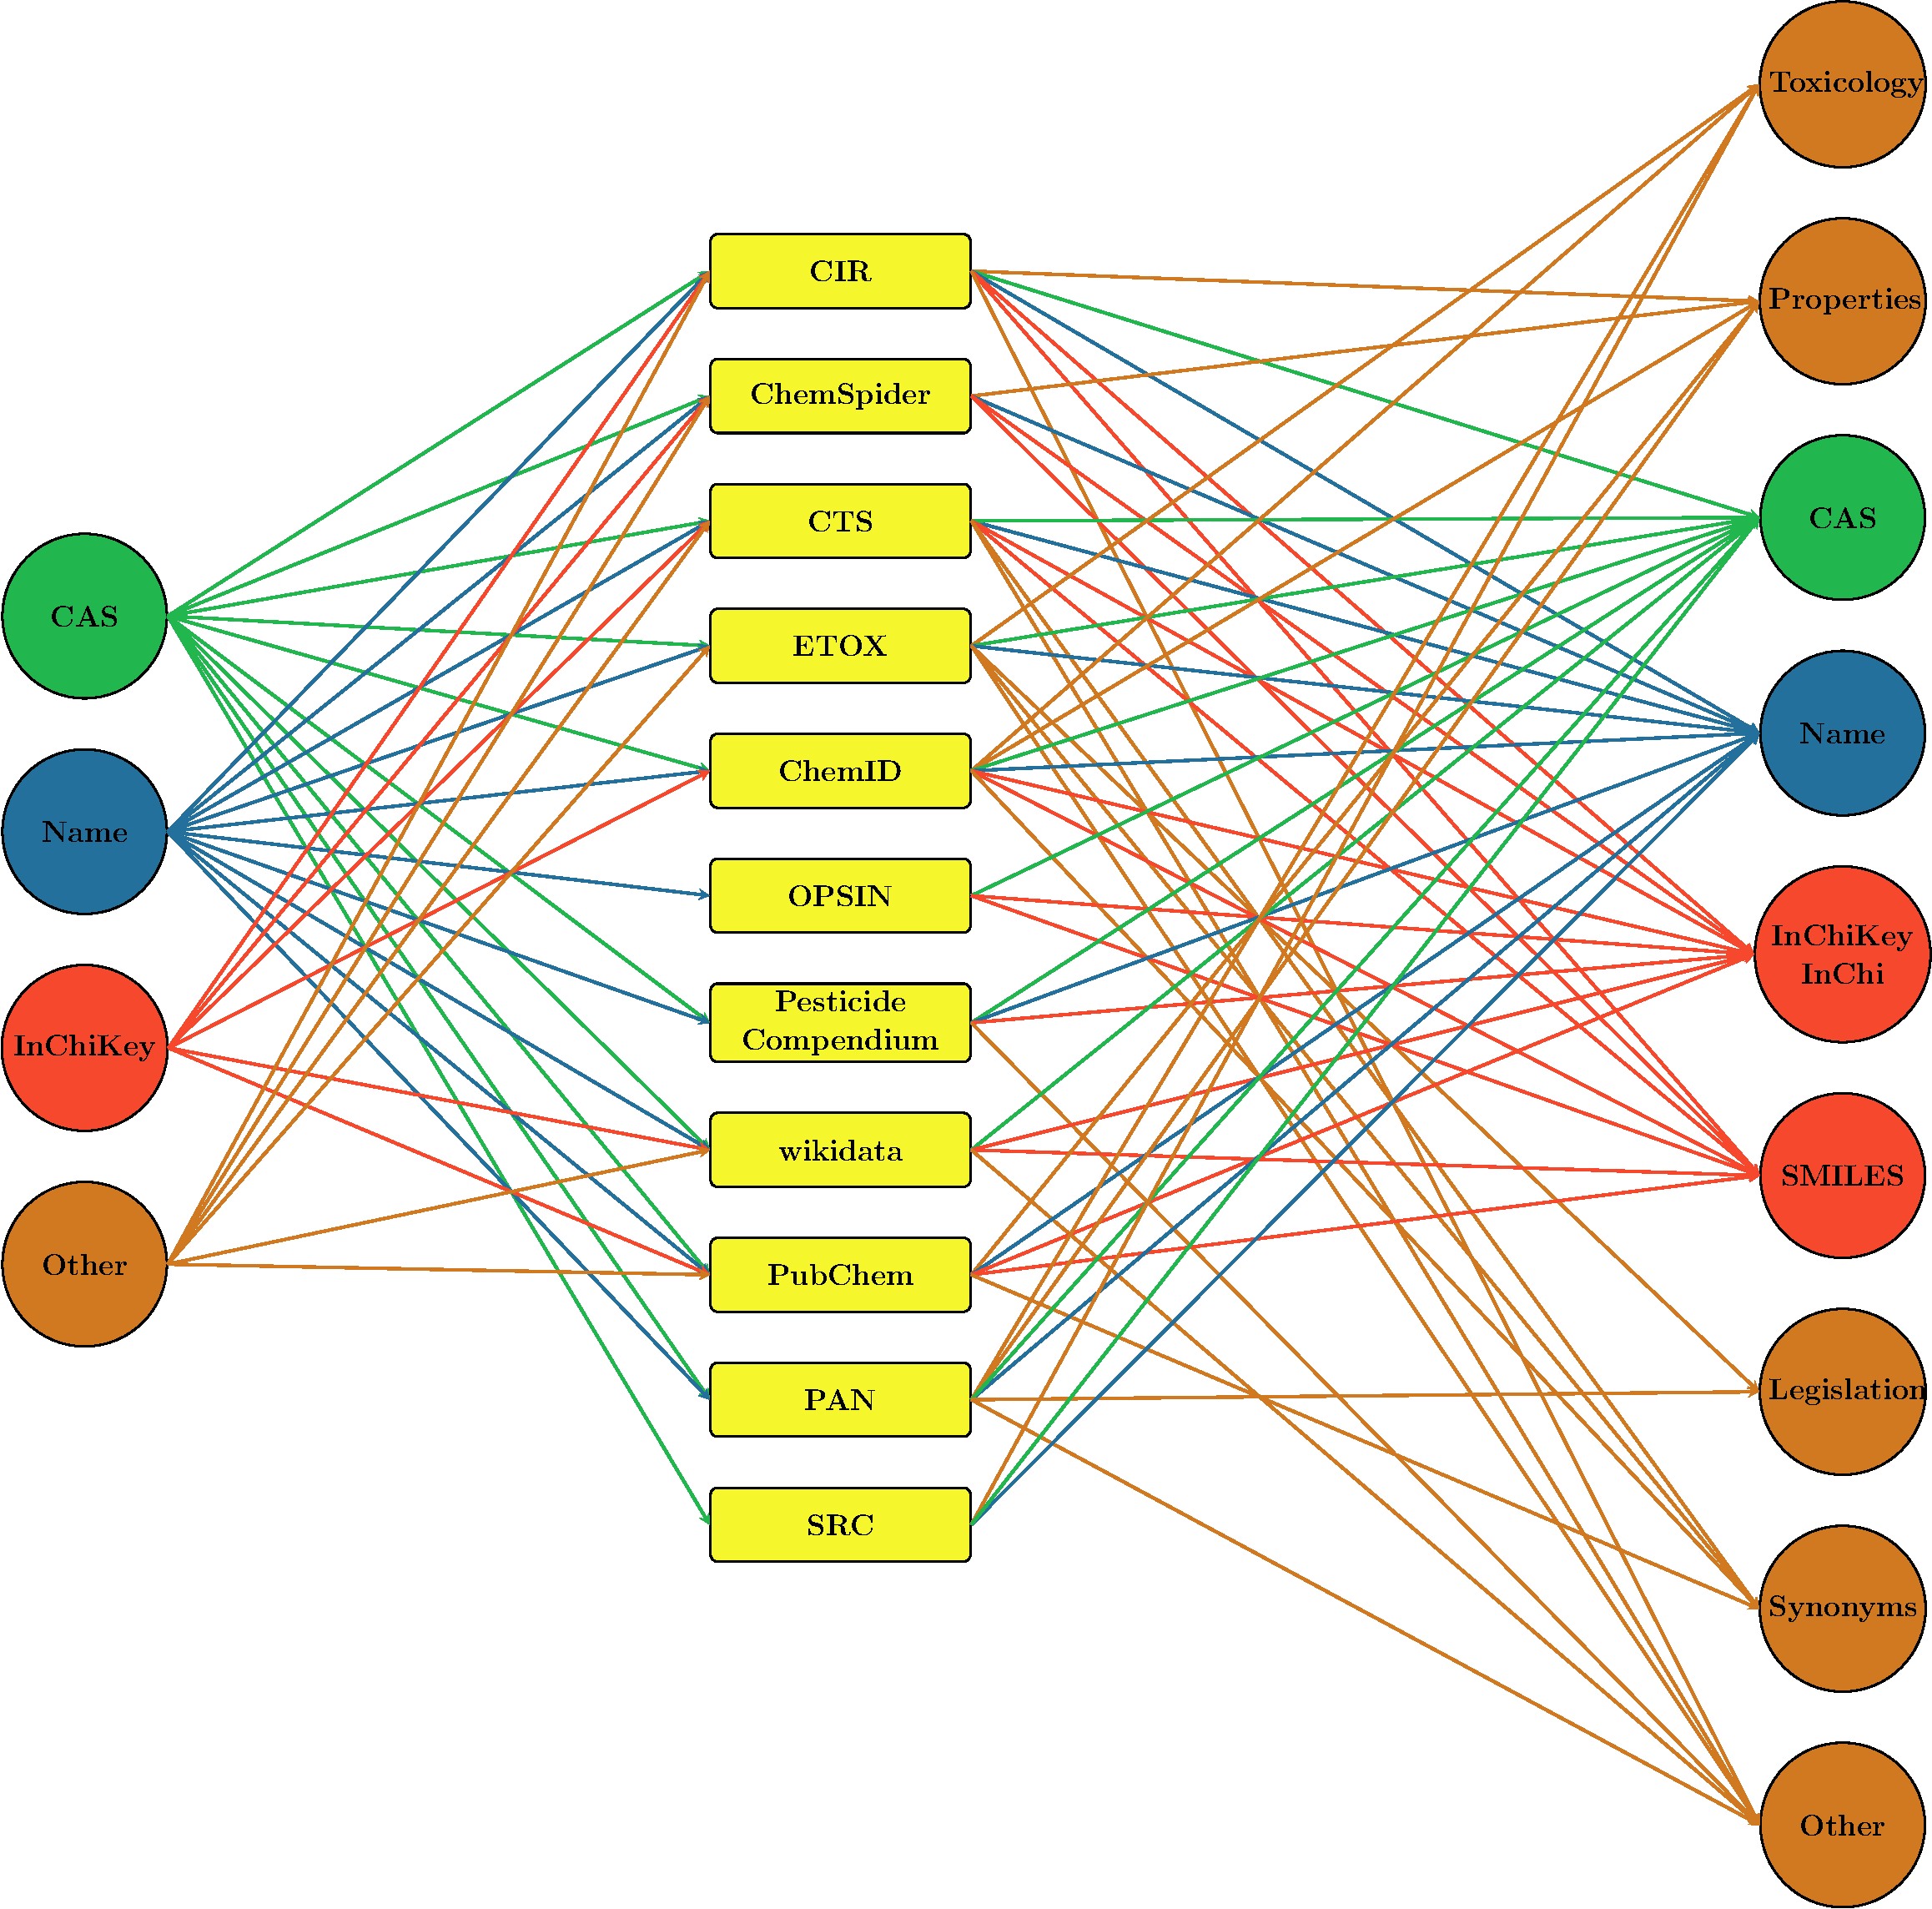
\includegraphics{fig1}
  \caption{Overview of current data sources. Input and output possibilities currently implemented in the package.}
  \label{fig:fig1}
\end{figure}


\section[Use cases]{Use cases}
\subsection[Installation]{Installation}
\pkg{webchem} can be easily installed from CRAN and loaded:
%
\begin{CodeChunk}
\begin{CodeInput}
R> install.packages("webchem")
R> library("webchem")
\end{CodeInput}
\end{CodeChunk}
%
The package is under active development. The latest development
version is available from GitHub and also permanently available at \citet{zenodo}.  This document has been created using \pkg{webchem}
version 0.5.0.


\subsection[Sample data sets]{Sample data sets}
To demonstrate the capabilities of \pkg{webchem} we use two small
publicly available real world data sets.  The data sets are only used
for purpose of demonstration, have been slightly preprocessed (not
shown) and are available through the package.

(i) \code{jagst}: This data set comprises environmental monitoring data of organic substances in the river Jagst, Germany, sampled in 2013.
The data is publicly available and can be retrieved from \citetalias{lubw_2016}.
It comprises concentrations  (in $\mathrm{\mu g~/~L}$) of  34 substances  on 13 sampling occasions.
First we load the data set and inspect the first six rows:
%
\begin{CodeChunk}
\begin{CodeInput}
R> data("jagst", package = "webchem")
R> head(jagst)
\end{CodeInput}
\begin{CodeOutput}
        date          substance value qual
1 2013-01-04 2,4-Dimethylphenol 0.006    <
2 2013-01-29 2,4-Dimethylphenol 0.006    <
3 2013-02-26 2,4-Dimethylphenol 0.006    <
4 2013-03-26 2,4-Dimethylphenol 0.006    <
5 2013-04-23 2,4-Dimethylphenol 0.006    <
6 2013-05-22 2,4-Dimethylphenol 0.006    <
\end{CodeOutput}
\end{CodeChunk}
%
This data set identifies substances only by substance names. Values below the limit of quantification (LOQ) are indicated by a qualifier column.

(ii) \code{lc50}: This data consists of median acute lethal concentration for the water flea \textit{Daphnia magna} in 48 h tests ($LC_{50, D.magna, 48h}$) of 124 insecticides.
The data has been retrieved from the EPA ECOTOX database \citep{epa_2016}.
%
\begin{CodeChunk}
\begin{CodeInput}
R> data("lc50", package = "webchem")
R> head(lc50)
\end{CodeInput}
\begin{CodeOutput}
       cas        value
4  50-29-3    12.415277
12 52-68-6     1.282980
15 55-38-9    12.168138
18 56-23-5 35000.000000
21 56-38-2     1.539119
36 57-74-9    98.400000
\end{CodeOutput}
\end{CodeChunk}
%
This data set identifies the substances only by CAS numbers.


\subsection[Query identifiers]{Query identifiers}
The \code{jagst} data set covers 34 substances that are identified by (German) names.
Merging and linking these to other tables is hampered by differences and ambiguity in compound names.

One possibility to resolve this, is to use different chemical
identifiers allowing easy identification.  There are several
identifiers available, e.g., registry numbers like CAS or EC, database
identifiers like PubChemCID \citep{Kim_2016} or ChemSpiderID
\citep{pence_chemspider:_2010}, line notations like SMILES
\citep{Weininger_1990}, InChI and InChIKey
\citep{Heller_McNaught_Pletnev_Stein_Tchekhovskoi_2015}.  In this
first example we query several identifiers to create a table that can
be used as (i) supplemental information to a research article or (ii)
to facilitate subsequent matching with other data.

As we are are dealing with German substance names we start to query ETOX for CAS registry numbers.
A common work flow when dealing with web resources is to 1) query a unique identifier of the source, 2) use this identifier to retrieve additional information and 3) extract the parts that are needed from the \proglang{R} object \citep{Chamberlain_Szocs_2013}.

First we search for ETOX internal ID numbers using the substance names:
%
\begin{CodeChunk}
\begin{CodeInput}
R> subs <- unique(jagst$substance)
R> ids <- get_etoxid(subs, match = "best")
R> head(ids)
\end{CodeInput}
\begin{CodeOutput}
  etoxid                           match distance                  query
1   8932     2,4-Dimethylphenol ( 8932 )        0     2,4-Dimethylphenol
2   8494 4-Chlor-2-methylphenol ( 8494 )        0 4-Chlor-2-methylphenol
3   <NA>                            <NA>     <NA>     4-para-nonylphenol
4   8397                Atrazin ( 8397 )        0                Atrazin
5   7240                 Benzol ( 7240 )        0                 Benzol
6   7331        Desethylatrazin ( 7331 )        0        Desethylatrazin
\end{CodeOutput}
\end{CodeChunk}
%
Only three substances could not be found in ETOX.  Here we specify
that only the \code{"best"} match (in terms of the Levenshtein
distance between query and results) is returned.  A manual check
confirms appropriate matches.  Other options include: \code{"all"} --
returns all matches; \code{"first"} -- returns only the first match
(not necessarily the best match); \code{"ask"} -- this enters an
interactive mode, where the user is asked for a choice if multiple
matches are found and \code{"na"} which returns \code{NA} in case of
multiple matches.

We use these data to retrieve basic information on the substances.
%
\begin{CodeChunk}
\begin{CodeInput}
R> etox_data <- etox_basic(ids$etoxid)
\end{CodeInput}
\end{CodeChunk}
%
\pkg{webchem} always returns a named list (one entry for each substance) and the available information content can be very voluminous.
Therefore, we provide extractor functions for the common identifiers: CAS, SMILES and InChIKeys.
%
\begin{CodeChunk}
\begin{CodeInput}
R> etox_cas <- cas(etox_data)
R> head(etox_cas)
\end{CodeInput}
\begin{CodeOutput}
       8668        8494        <NA>        8397        7240        7331 
 "105-67-9" "1570-64-5"          NA "1912-24-9"   "71-43-2" "6190-65-4" 
\end{CodeOutput}
\end{CodeChunk}
%
A variety of data are available and we cannot provide extractor
functions for each of those.  Therefore, if users need to extract
other data, they have to write simple extractor functions (see the
following examples).

In the same manner, we can now query other identifiers from another
source using these CAS numbers (see Figure~\ref{fig:fig1}), like
PubChem.
%
\begin{CodeChunk}
\begin{CodeInput}
R> cids <- get_cid(etox_cas)
R> pc_data <- pc_prop(cids, properties = "CanonicalSMILES")
R> pc_smiles <- smiles(pc_data)
\end{CodeInput}
\end{CodeChunk}
%
We can use SMILES to query ChemSpiderIDs and subsequently convert them to InChiKeys.
%
\begin{CodeChunk}
\begin{CodeInput}
R> csids <- get_csid(pc_smiles, from = "smiles")$csid
R> cs_inchikey <- cs_convert(csids, from = "csid", to = "inchikey")
\end{CodeInput}
\end{CodeChunk}
%
Finally, we combine the queried data into one data frame
%
\begin{CodeChunk}
\begin{CodeInput}
R> res <- data.frame(name = subs, cas = etox_cas, smiles = pc_smiles, 
+    cid = pc_data$CID, inchikey = cs_inchikey, csid = cs_data$csid, 
+    stringsAsFactors = FALSE)
\end{CodeInput}
\end{CodeChunk}
%
Note that in order to use the ChemSpider functions, a personal
authentication key is needed, which can be retrieved
from the ChemSpider web page.  Finally, we obtain a compound table
containing many different identifiers (Table~\ref{tab:comptable}),
allowing easy identification and merging with other data sets, e.g.,
the \code{lc50} data set based on CAS.

\begin{table}[t!]
\centering
\begin{tabular}{llllll}
  \hline
Name & CAS & SMILES & CID & InChIKey & CSID \\ 
  \hline
2,4-Dimethylphenol & 105-67-9 & CC1=CC(... & 7771 & KUFFULV... & 13839123 \\ 
  4-Chlor-2-methylphenol & 1570-64-5 & CC1=C(C... & 14855 & RHPUJHQ... & 14165 \\ 
  4-para-nonylphenol & -- & -- & -- & -- & -- \\ 
  Atrazin & 1912-24-9 & CCNC1=N... & 2256 & MXWJVTO... & 2169 \\ 
  Benzol & 71-43-2 & C1=CC=C... & 241 & UHOVQNZ... & 236 \\ 
  Desethylatrazin & 6190-65-4 & CC(C)NC... & 22563 & DFWFIQK... & 21157 \\ 
   \hline
\end{tabular}
\caption{Identifiers for the \code{jagst} data sets as queried with
  \pkg{webchem}. Only the first 6 entries are shown. For SMILES and
  InChIKey only the first 7 characters are shown. -- = not found.}
\label{tab:comptable}
\end{table}

\subsection[Toxicity of different pesticide groups]{Toxicity of different pesticide groups}
Another question we might ask is \emph{How does toxicity vary between
  insecticide groups?}  Answering this question would require tedious
lookup of insecticide groups for each of the 124 CAS numbers in the
\code{lc50} data set.  The Compendium of Pesticide Common Names
\citep{wood} contains such information and can be easily queried using
CAS numbers with \pkg{webchem}:
%
\begin{CodeChunk}
\begin{CodeInput}
R> aw_data <- aw_query(lc50$cas, type = "cas")
\end{CodeInput}
\end{CodeChunk}
%
To extract the chemical group from the retrieved data set, we write a simple extractor function and apply this to the retrieved data:
%
\begin{CodeChunk}
\begin{CodeInput}
R> igroup <- sapply(aw_data, function(y) y$subactivity[1])
R> igroup[1:3]
\end{CodeInput}
\begin{CodeOutput}
                                  50-29-3 
            "organochlorine insecticides" 
                                  52-68-6 
               "phosphonate insecticides" 
                                  55-38-9 
"phenyl organothiophosphate insecticides" 
\end{CodeOutput}
\end{CodeChunk}
%
Figure~\ref{fig:fig2} displays the result after additional data
cleaning (see the supplementary material for the full code).  Overall, it
took only 5 \proglang{R} statements to retrieve, clean and plot the
data using \pkg{ggplot2} \citep{ggplot2}.

\begin{figure}[t!]
  \centering
  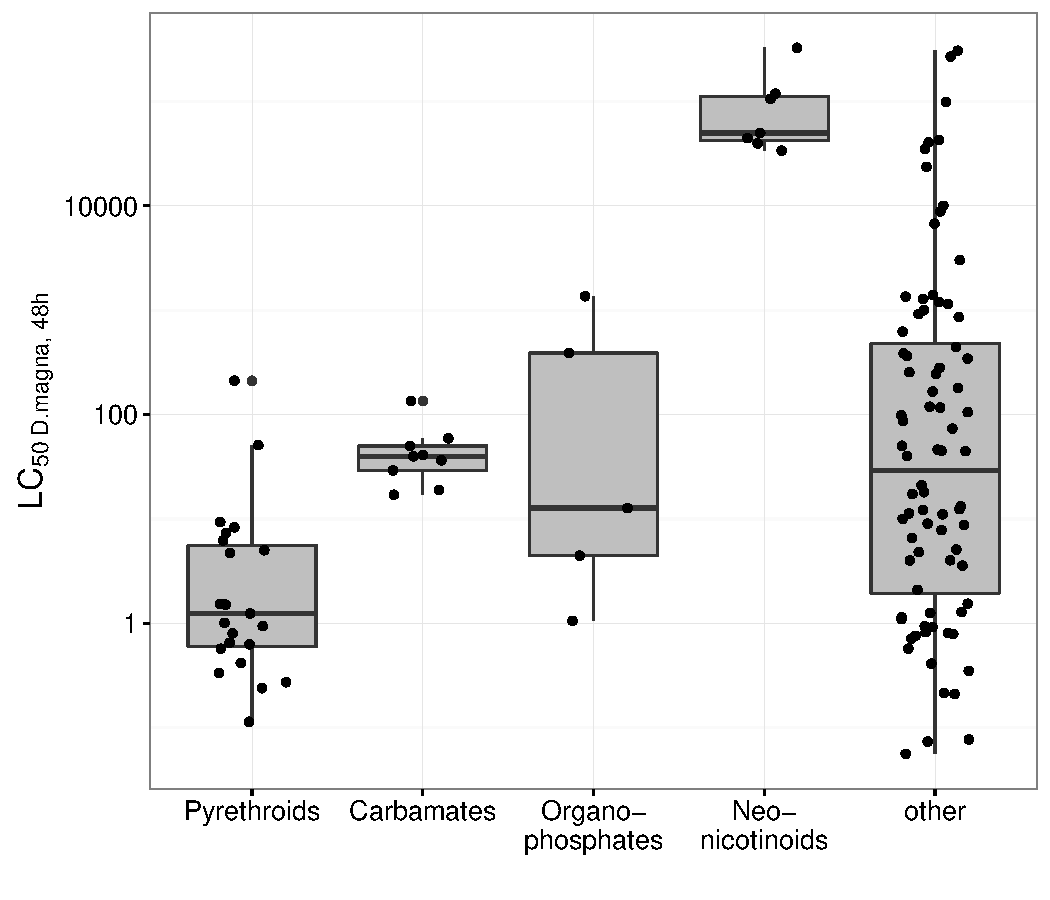
\includegraphics[width=0.7\textwidth, trim = 0 10 0 5, clip]{plot_lc50-1} 
\caption{Toxicity of different pesticide groups. LC\textsubscript{50}
  values have been retrieved from the EPA ECOTOX database, chemical groups
  from the Compendium of Pesticide Common Names \citep{wood}.}
\label{fig:fig2}
\end{figure}

\subsection[Identify common names and roles of chemicals]{Identify common names and roles of chemicals}
\pkg{webchem} can query the ChEBI database \citep{chebi} to retrieve common names and roles of chemicals on biota. Therefore, we first order the \code{lc50} data set by the three most toxic (i.e. lowest value) chemicals and then use \code{get_chebiid()} to retrieve ChEBI identifiers and substance names. The function returns a list of tables containing the ChEBI identifier, the chemical name, a search score and entity stars for the found entry. The searchscore is calculated by ChEBI and represents how well the query string matches one of the database entries. The entitystar column reflects the quality of the ChEBI data, also provided by the database.

\begin{CodeChunk}
\begin{CodeInput}
R> lite <- get_chebiid(lc50_3$cas)
R> lite <- do.call(rbind, lite) # bind to data.frmae
R> lite$cas <- rownames(lite)
R> lite$chebiasciiname[4] <- "tefluthrin" # erronous result
\end{CodeInput}
\end{CodeChunk}

We can now use the ChEBI identifiers to query the complete entitiy by using \code{chebi_comp_entity()}. From the result, we extract the parents table and refine the data to chemical roles. Subsequently, we prepare the query result and merge the data with the \code{lite} object to include the CAS numbers (i.e. our initial query strings) to the result.

\begin{CodeChunk}
\begin{CodeInput}
R> comp <- chebi_comp_entity(lite$chebiid) # ChEBI ids
R> comp <- do.call(rbind, lapply(comp, `[[`, "parents")) # extract parents table
R> comp$chebiid <- gsub('\\.[0-9]+', '', rownames(comp))
R> comp <- comp[ comp$type == "has role", ] # refine to chemical roles
R> role <- aggregate(chebiName ~ chebiid,
                     data = comp,
                     FUN = function(x) paste0(x, collapse = ', '))
R> merge(lite[ names(lite) %in% c('cas', 'chebiid', 'chebiasciiname') ],
         role,
         by = 'chebiid')
\end{CodeInput}
\end{CodeChunk}

In doing so we retrieve Table~\ref{tab:chebi}, which provides information on the individual roles of the chemicals and we observe that, for example ethion, the most toxic pesticide towards \textit{D. magna} in our table is designed to be used as an acari- and insecticide, which inhibts the acetylcholinesterase enzyme.

\begin{table}[t!]
\centering
\begin{tabular}{p{2cm}p{2cm}p{8cm}}
  \hline
  cas & name & roles \\
  \hline
  563-12-2 & ethion & insecticide \newline environmental contaminant \newline EC 3.1.1.7 (acetylcholinesterase) inhibitor \newline acaricide \newline agrochemical \\
  96182-53-5 & tebupirimfos & EC 3.1.1.7 (acetylcholinesterase) inhibitor \\
  3383-96-8 & temephos & EC 3.1.1.7 (acetylcholinesterase) inhibitor \newline acaricide \newline agrochemical \newline ectoparasiticide \\
\hline
\end{tabular}
\caption{CAS numbers, names and chemical roles for the three most toxic substances towards \textit{D. magna} according to ChEBI.}
\label{tab:chebi}
\end{table}

\subsection[Querying partitioning coefficients]{Querying partitioning coefficients}
Some data sources also provide data on chemical properties that can be
queried.  Here we query for the \code{lc50} data predicted
$\mathrm{log}~P_{oct/wat}$ from the PubChem database to build a
simple quantitative structure-activity relationship (QSAR) to predict
toxicity. The resulting data and model are displayed in Figure~\ref{fig:fig3}.
%
\begin{CodeChunk}
\begin{CodeInput}
R> cid <- get_cid(lc50$cas)
R> pc_data <- pc_prop(cid)
R> lc50$logp <- pc_data$XLogP
\end{CodeInput}
\end{CodeChunk}
%

\begin{figure}[t!]
  \centering
  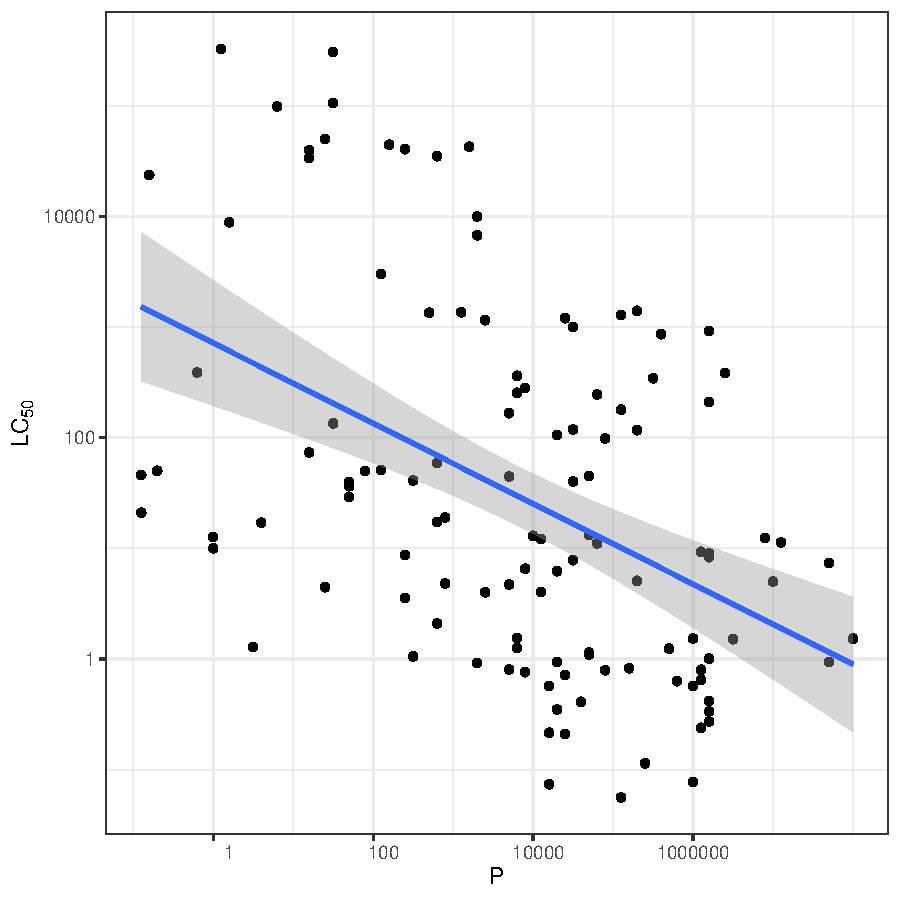
\includegraphics[width=0.7\textwidth]{plot_qsar-1} 
  \caption{Simple QSAR for predicting log LC\textsubscript{50} of
    pesticides by $\mathrm{log}~P$.  $\mathrm{log}~P$ values have been
    retrieved from the Pubchem database (118 estimated data and 6 substances without data).  Blue line
    indicates the regression model
    ($\mathrm{log~LC}_{50} = 2.86\ensuremath{-0.36}~\mathrm{log}~P$,
    RMSE = 1.47).}
\label{fig:fig3}
\end{figure}


\subsection[Regulatory information]{Regulatory information}
Regulatory information is particularly of interest if concentrations
exceed national thresholds.  In the European Union (EU) the Water
Framework Directive (WFD; \citealt{wfd2000directive}) defines
Environmental Quality Standards (EQS).  Similarly, the U.S.\ and
Canadian EPA and the WHO define Quality Standards.  Information on
these standards can be queried with \pkg{webchem} from the PAN
Pesticide Database (using \code{pan\_query()}) and from ETOX (using
\code{etox\_targets()}).

In this example we search for the minimum EQS for the EU for the
compounds in the \code{jagst} data set, join these with measured
concentrations and evaluate whether exceedances occurred.

We re-use the above queried ETOX-IDs to obtain further information
from ETOX, namely the MAC-EQS:
% 
\begin{CodeChunk}
\begin{CodeInput}
R> eqs <- etox_targets(ids$etoxid)
R> ids$mac <- sapply(eqs, function(y) {
+    if (length(y) == 1 && is.na(y)) {
+      return(NA) 
+    } else {
+      res <- y$res
+      min(res[res$Country_or_Region == "EEC / EU" & 
+        res$Designation == "MAC-EQS", "Value_Target_LR"])
+    }
+  })
\end{CodeInput}
\end{CodeChunk}
%
Again, the returned information is humongous and we encourage users to study the returned objects and description of the data source.
Here, the column \code{Designation} defines the type of EQS and \code{Value_Target_LR} contains the value.
Unfortunately, we only found MAC-EQS values for 6 substances:
%
\begin{CodeChunk}
\begin{CodeInput}
R> (mac <- with(ids, ids[!is.na(mac) & is.finite(mac), c("etoxid", "query",
+    "mac")]))
\end{CodeInput}
\begin{CodeOutput}
   etoxid       query    mac
4    8397     Atrazin  2.000
5    7240      Benzol 50.000
11   8836     Irgarol  0.016
12   7442 Isoproturon  1.000
38   7571     Simazin  4.000
29   8756   Terbutryn  0.034
\end{CodeOutput}
\end{CodeChunk}
%
The \code{get_etoxid()} function used to search ETOX-IDs returns also
the original substance name (\code{query}), so that we can easily join
the table with MAC values with the measurements table:
% 
\begin{CodeChunk}
\begin{CodeInput}
R> jagst_eqs <- merge(jagst, mac, by.x = "substance", by.y = "query")
R> head(jagst_eqs)
\end{CodeInput}
\begin{CodeOutput}
  substance       date  value qual etoxid mac
1   Atrazin 2013-09-10 0.0068    =   8397   2
2   Atrazin 2013-10-08 0.0072    =   8397   2
3   Atrazin 2013-03-26 0.0040    =   8397   2
4   Atrazin 2013-04-23 0.0048    =   8397   2
5   Atrazin 2013-06-18 0.0048    =   8397   2
6   Atrazin 2013-07-16 0.0052    =   8397   2
\end{CodeOutput}
\end{CodeChunk}
%
Finally, we can compare the measured value to the MAC, which reveals that there have been no exceedances of these 6 compounds.




\subsection[Utility functions]{Utility functions}
Furthermore, \pkg{webchem} provides also basic functions to check identifiers that can be used for data quality assessment.
The functions either use simple formatting rules,
%
\begin{CodeChunk}
\begin{CodeInput}
R> is.inchikey("BQJCRHHNABKAKU-KBQPJGBKS-AN")
\end{CodeInput}
\begin{CodeOutput}
Hyphens not at position 15 and 26.
\end{CodeOutput}
\begin{CodeOutput}
[1] FALSE
\end{CodeOutput}
\begin{CodeInput}
R> is.cas("64-17-6")
\end{CodeInput}
\begin{CodeOutput}
Checksum is not correct! 5 vs. 6
\end{CodeOutput}
\begin{CodeOutput}
[1] FALSE
\end{CodeOutput}
\end{CodeChunk}
%
or web resources like ChemSpider
%
\begin{CodeChunk}
\begin{CodeInput}
R> is.inchikey("BQJCRHHNABKAKU-KBQPJGBKSA-5", type = "chemspider")
\end{CodeInput}
\begin{CodeOutput}
[1] FALSE
\end{CodeOutput}
\end{CodeChunk}
%
\section[Discussion]{Discussion}
\subsection[Related software]{Related software}
Within the \proglang{R} ecosystem, there are only a few similar
projects: \pkg{rpubchem} \citep{rpubchem_2014} provides an interface
to PubChem.  Similarly, \pkg{ChemmineR} \citep{chemminer_2008}, a
mature chemo-informatics package, provides an interface to PubChem.
\pkg{webchem} does not provide any chemo-informatic functionality, but
integrates access to many data sources.  \pkg{WikidataR}
\citep{wikidatar_2016} provides an interface to wikidata that could be
used to retrieve chemical data from Wikipedia.  However, it does not
provide predefined methods for chemical data like \pkg{webchem}.
Within the \proglang{Python} \citep{python} ecosystem the libraries
\pkg{PubChempy} \citep{pubchempy}, \pkg{ChemSpiPy} \citep{chemspipy}
and \pkg{CIRpy} \citep{cirpy} are available for similar tasks as those
outlined here.  \pkg{webchem} is not specialized and tries to
integrate many data sources and for some of these it provides a unique
programmatic interface.  The Chemical Translation Service
\citep{Wohlgemuth_Haldiya_Willighagen_Kind_Fiehn_2010}, which is also
one of the sources that can be queried, allows batch conversion of
chemical identifiers.  However, it does not provide access to other
data (experimental, modeled or regulatory data).


\subsection[Open Science]{Open Science}
An increasing number of scientific data is becoming publicly available
\citep{Gewin_2016, Reichman_Jones_Schildhauer_2011,Boyle_Guha_2011},
either in public data repositories or as supplements to publications.
To be usable for other researchers chemical compounds should be
properly identified, not only by chemical names but also with
accompanying identifiers like InChIKey, SMILES and authority-assigned
identifiers.  \pkg{webchem} provides an easy way to create such meta
tables as shown in Table~\ref{tab:comptable} and facilitates chemical
data availability to researchers.  However, good quality of data is
crucial for every analysis \citep{Stieger_2014} and additional effort
and methods are needed to validate data quality.

\subsection[Further development]{Further development}
We have outlined only a few use cases that will likely be useful for
many researchers.  Given the huge amount of publicly available
information, many other possibilities can be envisioned.
\pkg{webchem} is currently under active development and several other
data sources have not been implemented yet but may be in the future.
GitHub makes contributing easy and we strongly encourage contribution
to the package.  Moreover, comments, feedback and feature requests are
highly welcome.


\section[Conclusions]{Conclusions}
Researchers need to have easy access to global knowledge on chemicals.
\pkg{webchem} can save \emph{hundreds of working hours} gathering
this knowledge \citep{Munch_Galizia_2016}, so that researchers can
focus on other tasks.


\section*{Acknowledgments}
We thank all resource maintainers for their work making their data
open to the public.  We thank Johannes Ranke and Daniel M{\"u}nch for
their contributions to the \pkg{webchem} package, as well as all users who
provided feedback and feature requests.  We are grateful to Zacharias
Steinmetz for valuable comments on the manuscript.


\bibliography{ref}

\end{document}
